\documentclass[conference]{IEEEtran}
\IEEEoverridecommandlockouts
% The preceding line is only needed to identify funding in the first footnote. If that is unneeded, please comment it out.
\usepackage{amsmath,amssymb,amsfonts}
\usepackage{algorithmic}
\usepackage{graphicx}
\usepackage{float} 
\usepackage{subfigure}
\usepackage{textcomp}
\usepackage{xcolor}
\usepackage{CJK}
%\usepackage[UTF8]{ctex} % 加这个会变成中文,不加就显示不出来
\usepackage{booktabs}
\usepackage{caption}
\usepackage[colorlinks]{hyperref}
\usepackage{cite}
\usepackage{amsmath,amssymb,amsfonts}
\usepackage{algorithmic}
\usepackage{graphicx}
\usepackage{textcomp}
\usepackage{xcolor}
\def\BibTeX{{\rm B\kern-.05em{\sc i\kern-.025em b}\kern-.08em
    T\kern-.1667em\lower.7ex\hbox{E}\kern-.125emX}}
\begin{document}

\title{Detection and Classification of Pulmonary Nodules
}

    \author{\IEEEauthorblockN{1\textsuperscript{st} Given Name Surname}
    \IEEEauthorblockA{\textit{dept. name of organization (of Aff.)} \\
    \textit{name of organization (of Aff.)}\\
    City, Country \\
    email address or ORCID}
\and
\IEEEauthorblockN{2\textsuperscript{nd} Given Name Surname}
\IEEEauthorblockA{\textit{dept. name of organization (of Aff.)} \\
\textit{name of organization (of Aff.)}\\
City, Country \\
email address or ORCID}
\and
\IEEEauthorblockN{3\textsuperscript{rd} Given Name Surname}
\IEEEauthorblockA{\textit{dept. name of organization (of Aff.)} \\
\textit{name of organization (of Aff.)}\\
City, Country \\
email address or ORCID}
\and
\IEEEauthorblockN{4\textsuperscript{th} Given Name Surname}
\IEEEauthorblockA{\textit{dept. name of organization (of Aff.)} \\
\textit{name of organization (of Aff.)}\\
City, Country \\
email address or ORCID}
\and
\IEEEauthorblockN{5\textsuperscript{th} Given Name Surname}
\IEEEauthorblockA{\textit{dept. name of organization (of Aff.)} \\
\textit{name of organization (of Aff.)}\\
City, Country \\
email address or ORCID}
\and
\IEEEauthorblockN{6\textsuperscript{th} Given Name Surname}
\IEEEauthorblockA{\textit{dept. name of organization (of Aff.)} \\
\textit{name of organization (of Aff.)}\\
City, Country \\
email address or ORCID}
}

\maketitle
\begin{CJK}{UTF8}{gbsn}
\begin{abstract}
    Pulmonary nodule detection and
    classification represent two of the most common tasks in the computer
    aided analysis of chest CT images. Methods have been proposed for each
    task with deep learning based methods heavily favored recently.
    However training deep learning models to solve each task separately may be
    sub-optimal - resource intensive and without the benefit of feature sharing. 
\end{abstract}

\begin{IEEEkeywords}
    pulmonary nodule detection and classification
    , deep convolutional neural network
\end{IEEEkeywords}

\section{Introduction}
Pulmonary nodules are defined as focal, quasi-circular, dense or asfirm lung shadows with imaging findings of diameter $\leq$ 3 cm. \cite{wang2019}
CT is the most important means for diagnosis, follow-up and efficacy evaluation of pulmonary nodules, but there is radiation during scanning, which has certain effects on human body.In general, low-dose CT can be used, at one-fifth or less of the conventional dose, with minimal impact on the human body.The normal population is recommended to have a yearly scan.
Thin-section CT, enhanced CT, MAGNETIC resonance imaging, positron emission computed tomography (PET) and other imaging examinations can be used to analyze the properties of pulmonary nodules from the aspects of morphology and metabolic function, which is of great reference value for the diagnosis of pulmonary nodules.But it's not a diagnosis.Therefore, from the perspective of diagnosis, clinical diagnosis can be made by analyzing the cell or tissue samples obtained from pulmonary nodules through bronchoscopy, percutaneous puncture, surgical methods, etc.
\section{Literature Review}



\section{Model}
\subsection{Preprocess the Data}
The data of LUNA16 came from a larger data set, LIDC-IDRI, which had a total of 1018 CT scans, or 1018 cases. Each CT image had a label file in XML format. The data of this data set came from seven different 
academic institutions, which used different scanners and related parameters. In LIDC - IDRI data set, there are three areas will be marked, nodules $\textgreater$ 3 mm in diameter, diameter $\textless $ 3 mm nodules and the nodules
 (but lung distortion area), return to LUNA16, in 888 CT, a total of 36378 nodes were marked (LIDC - IDRI annotation), in LUNA16, only diameter $\textgreater$ 3 mm nodules as sample, diameter $\textless $ 3 mm nodules and the nodules are not included. 
 To train the data, the first step is to genrate the mask of pulmonary nodules. The annotations.csv annoatates the coordinates of X, Y, Z as well as the diameter of pulmonary nodules, with these data, the cube area is generated, and finally the Mask image file is output.
The second step is image denoising. We set the window width and window level (-1000,600) to remove the noise in the CT image, such as bone highlights, metal lines of the CT bed, etc., and normalize the image to (0,1). The third step is to crop the picture to the same size.
The CT image with a layer thickness greater than 1mm and the corresponding Mask image were sampled with interpolation (linear interpolation method was used for CT image and nearest-neighbor interpolation method for Mask image), and the layer thickness after interpolation sampling was 1mm.
The size of Patch area (96,96,16) in CT image and Mask image was taken according to a certain step length, and the valid Patch Mask image and corresponding Pactch image were judged and retained. The final step is to prepare benign and malignant pulmonary nodules classification data.Coordinates are read from the candidates.csv file, and images of the size 
of (48,48,48) are taken as candidate pulmonary nodules images centering on this coordinate, and the images are divided into two categories according to the label value (0 or 1).
After doing these steps, we have data that we can train with. And we found that There were 1,351 pulmonary nodules and 549,714 non-pulmonary nodules.There's a huge difference between positive and negative samples.Therefore, we performed data enhancement processing on the data, and randomly sampled 20$\%$ of the data from 549714 non-pulmonary nodules images, which were enlarged by 40 times (rotation, translation, inversion, etc.) for 1,351 pulmonary nodules images.
A total of 601 of the 888 cases had pulmonary nodules in the CT data, and a total of 16,475 patches were taken out from the 601 cases.We chose 80 percent of the data for training and 20 percent for testing.
\begin{figure}[htbp]
    \centerline{
\includegraphics[scale=0.5]{1.jpg}}
    \caption{Accorind to cadidattes.csv, we generate the mask of pulmonary nodule}
    \label{fig1}
    \end{figure}
\subsection{Nodule Detection}
We use 3DVNet network model to achieve detection. It could be seen in \ref{fig2}. 
And to illustrate, the following points should be noted:
\begin{itemize}
    \item The Conv layer connecting the output layer adopts the convolution kernel of 1x1x1 size, while the remaining Conv layer adopts the convolution kernel of 3x3x3 size.
    \item 3dMaxPooling layer is adopted in the pooling layer.
    \item The Upsample layer is implemented by the deconvolution layer.
    \item Concate layer splices the results of Conv layer and Upsample layer in the decoding network.
\end{itemize}
\begin{figure}[htbp]
    \centerline{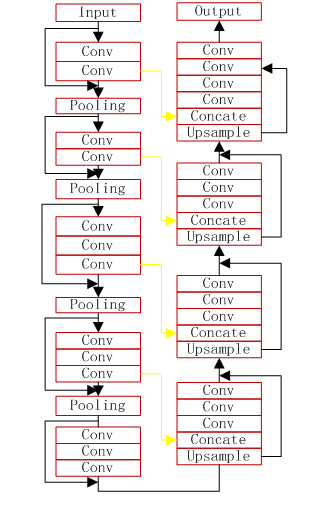
\includegraphics[scale=0.5]{3dVNet.png}}
    \caption{Network structure of 3dVNet}
    \label{fig2}
    \end{figure}
What's more, The residual connection is also used to prevent the gradient disappearing during the training. Our parameter is set as learning rate is 0.001, Batchsize is 6, and epoches is 10.
And the loss function is as followed:
\begin{equation}\operatorname{dice}=\frac{2^{*} \operatorname{abs}\left(A^{*} B\right)}{A^{2}+B^{2}}\end{equation}
The result could be seen in \ref{fig3}
\begin{figure}[htbp]
    \centerline{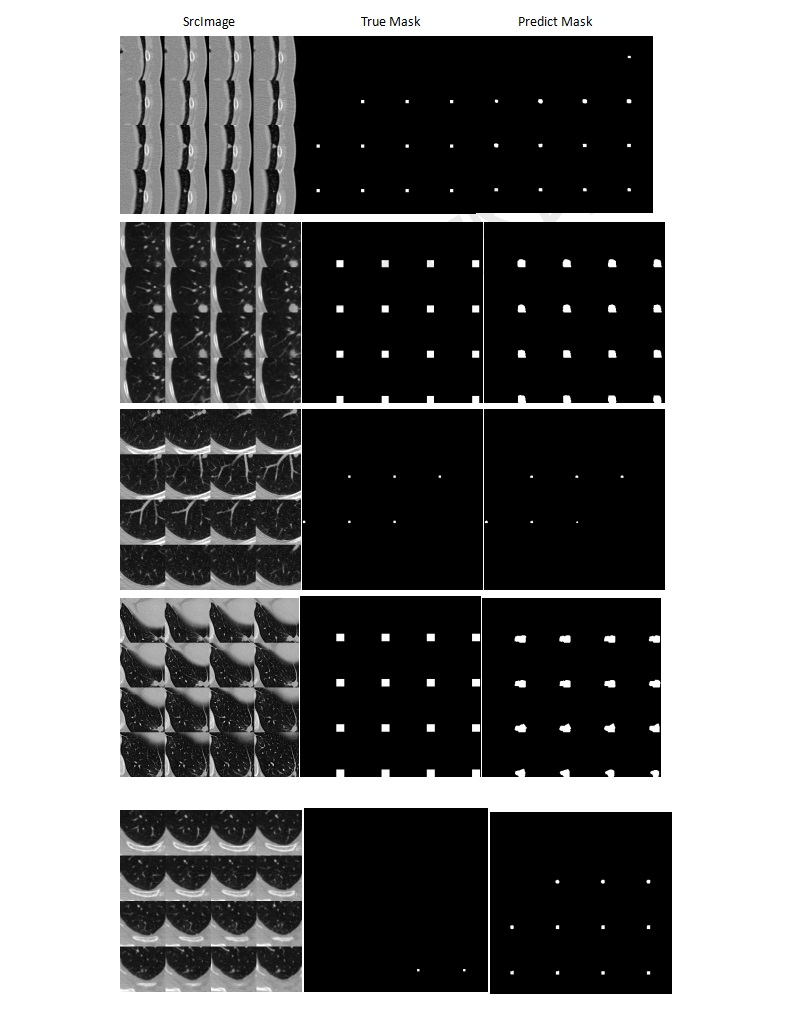
\includegraphics[scale=0.5]{segImage.jpg}}
    \caption{Our result of detection on the test data. The original image is predicted and compared with the gold standard image.The original image is shown on the left, the gold standard image is shown in the middle, and the predicted image is shown on the right.}
    \label{fig3}
    \end{figure}
\subsection{Nodule Classify}
Classification network is a mature network, and there are many network models with good performance.We use an improved version of THE VGG network to achieve benign and malignant classification. The structure could be seen in\ref{fig4}.And to illustrate, the following points should be noted:
\begin{itemize}
    \item All Conv layers adopt 3x3x3 convolution kernel.
    \item 3dMaxPooling layer is adopted in the pooling layer.
    \item The FC layer is the full connection layer. The first FC USES Relu activation function, while the second FC USES Softmax activation function.
\end{itemize}
\begin{figure}[htbp]
    \centerline{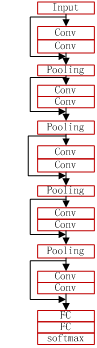
\includegraphics[scale=0.5]{ResVGGNet.png}}
    \caption{The structre of ResVGGNet}
    \label{fig4}
    \end{figure}
The residual connection is also used to prevent the gradient disappearing during the training. Our parameter is set as learning rate is 0.001, Batchsize is 32, and epoches is 5.
And we adopt cross entropy function as loss function.
\begin{equation}\operatorname{loss}=-\sum_{i=1}^{n} y_{i}^{*} \log \left(y_{i_{-}}\right)\end{equation}
\section{Results}
The result of detection could be seen in \ref{fig3} and \ref{fig5}. And the accuracy could reach to 62$\%$ and it is still going up. Due to the 
time limited, we cannot train it completely.\\
\begin{figure}[htbp]
    \centerline{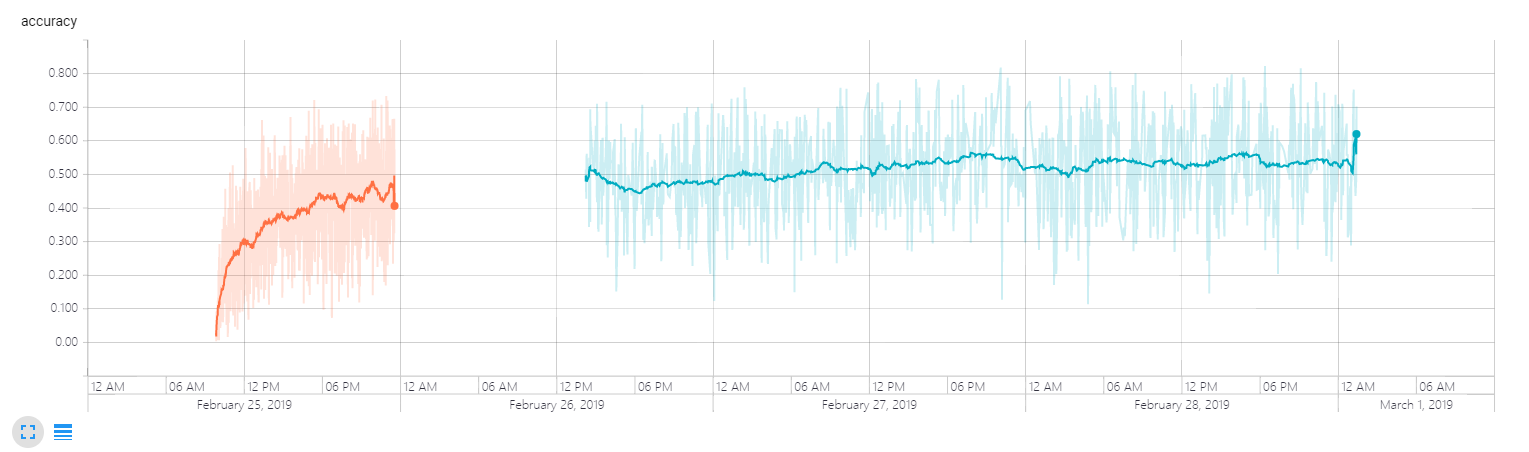
\includegraphics[scale=0.2]{segaccuracy.PNG}}
    \caption{The result of detection.The red line is the first training, and the blue line is the result of the first training}
    \label{fig5}
    \end{figure}
The result of classification could be seen in \ref{fig6}. By analyzing the confounding matrix, the overall accuracy rate of the classifier is 98.73$\%$
, the false positive rate is 1.718$\%$ and the omission rate is 0.394$\%$.
\begin{figure}[htbp]
    \centerline{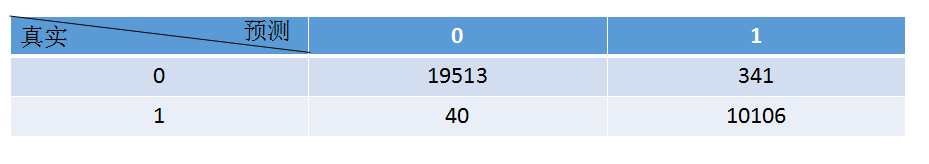
\includegraphics[scale=0.3]{ConfusionMatrix.PNG}}
    \caption{The result of detection.The red line is the first training, and the blue line is the result of the first training}
    \label{fig6}
    \end{figure}
\section{Future Studies}
Due to the time and device limited, we only use one model to achieve the detection and classification of pulmonary nodules. With the research of convolutional networks,
more models are put award. And in the future we will use these models to improve accuracy of classification and detection.


\section*{Acknowledgment}
Thanks very much for my group members in this internship. I would also like to express my gratitude for Dr Teoh Teik Toe for his discussion of topic selection and guidance on some issues in the early stage of my project. I also have a new dream school, and I hope I can meet the graduate student in NTU again.

% \section*{References}

% Please number citations consecutively within brackets \cite{b1}. The 
% sentence punctuation follows the bracket \cite{b2}. Refer simply to the reference 
% number, as in \cite{b3}---do not use ``Ref. \cite{b3}'' or ``reference \cite{b3}'' except at 
% the beginning of a sentence: ``Reference \cite{b3} was the first $\ldots$''

% Number footnotes separately in superscripts. Place the actual footnote at 
% the bottom of the column in which it was cited. Do not put footnotes in the 
% abstract or reference list. Use letters for table footnotes.

% Unless there are six authors or more give all authors' names; do not use 
% ``et al.''. Papers that have not been published, even if they have been 
% submitted for publication, should be cited as ``unpublished'' \cite{b4}. Papers 
% that have been accepted for publication should be cited as ``in press'' \cite{b5}. 
% Capitalize only the first word in a paper title, except for proper nouns and 
% element symbols.

% For papers published in translation journals, please give the English 
% citation first, followed by the original foreign-language citation \cite{b6}.


% \begin{thebibliography}{00}
% \bibitem{b1} 王静. 肺结节,我们该如何对待[J]. 家庭健康, 2019, 000(003):20.
% \bibitem{b2} J. Clerk Maxwell, A Treatise on Electricity and Magnetism, 3rd ed., vol. 2. Oxford: Clarendon, 1892, pp.68--73.
% \bibitem{b3} I. S. Jacobs and C. P. Bean, ``Fine particles, thin films and exchange anisotropy,'' in Magnetism, vol. III, G. T. Rado and H. Suhl, Eds. New York: Academic, 1963, pp. 271--350.
% \bibitem{b4} K. Elissa, ``Title of paper if known,'' unpublished.
% \bibitem{b5} R. Nicole, ``Title of paper with only first word capitalized,'' J. Name Stand. Abbrev., in press.
% \bibitem{b6} Y. Yorozu, M. Hirano, K. Oka, and Y. Tagawa, ``Electron spectroscopy studies on magneto-optical media and plastic substrate interface,'' IEEE Transl. J. Magn. Japan, vol. 2, pp. 740--741, August 1987 [Digests 9th Annual Conf. Magnetics Japan, p. 301, 1982].
% \bibitem{b7} M. Young, The Technical Writer's Handbook. Mill Valley, CA: University Science, 1989.
% \end{thebibliography}
% \vspace{12pt}
% \color{red}
% IEEE conference templates contain guidance text for composing and formatting conference papers. Please ensure that all template text is removed from your conference paper prior to submission to the conference. Failure to remove the template text from your paper may result in your paper not being published.
\bibliographystyle{ieeetr}
\bibliography{ref.bib}
\end{CJK}
\end{document}
